\documentclass{standalone}

\usepackage{circuitikz}

\begin{document}

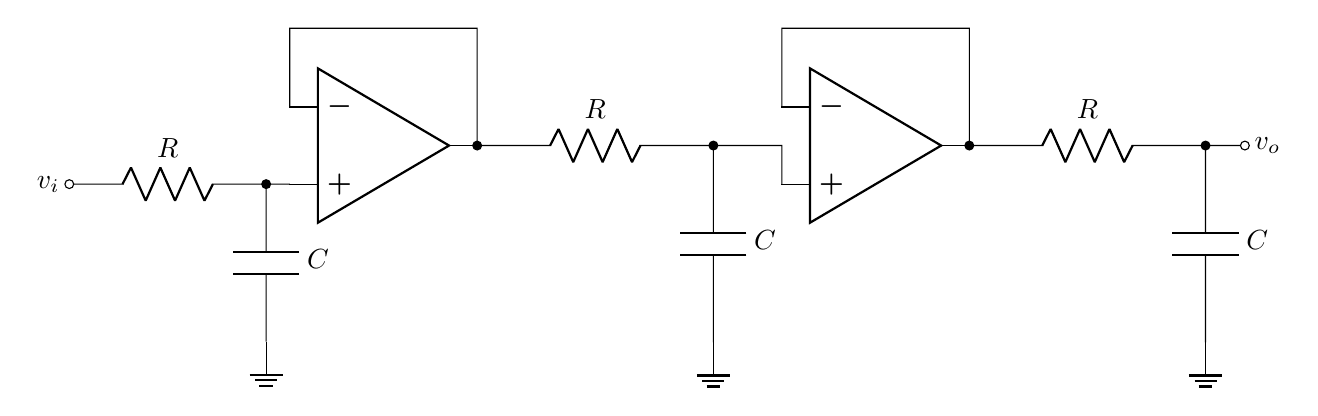
\begin{tikzpicture} \draw
	(0,0) node[op amp] (opamp1) {}
	(opamp1.+) to [short, -*] ++(-0.3,0) coordinate(node1)
	(node1) to [R, l_=$R$, -o] ++(-2.5,0) node[left]{$v_i$}
	(node1) to [C, l=$C$] ++(0,-2) node[ground] {}
	(opamp1.-) to [short] ++(0,1) to [short] ++(2.38,0) to (opamp1.out)
	(opamp1.out) to[R, l=$R$, *-] ++(3,0) coordinate(node2)
	(node2) to[C, l=$C$, *-] ++(0,-2.5) node[ground] {}
	%de fase%
	(6.25,0) node[op amp] (opamp2) {}
	(node2) -| (opamp2.+)
	(opamp2.-) to [short] ++(0,1) to [short] ++(2.38,0) to (opamp2.out)
	(opamp2.out) to [R, l=$R$, *-] ++(3,0) coordinate(node3)
	(node3) to [C, l=$C$, *-] ++(0, -2.5) node[ground]{}
	(node3) to [short, -o] ++(0.5,0) node[right]{$v_o$}
	;
\end{tikzpicture}

\end{document}